% =====================================================================
% figD  — R/ggplot2 -> tikzDevice (parallel to ../figures-tex/figD_editor.tex)
% Canonical-JSON-only. Regenerate: Rscript figures/make_figures_ieee.R
% Provenance (JSON path :: field = plotted value), one line per series:
% SOURCE: results/C3_null_ft_L8.json :: aggregate.within_probe_mean_across_seeds [y=rho] = 0.0239
% SOURCE: results/gate_llama1b_ft_cf_L8_s0.json :: KNOWN_PROBES.mean_damage_logit [x=mean damage] = 18.1196
% SOURCE: results/C3_null_ftkl_L8_v2.json :: aggregate.within_probe_mean_across_seeds [y=rho] = 0.1322
% SOURCE: results/gate_llama1b_ftkl_cf_L8_s0.json :: KNOWN_PROBES.mean_damage_logit [x=mean damage] = 15.2025
% SOURCE: results/C1_mechanism_sc_table.json :: groups[llama1b,L8].within_probe_rho_C [y=rho] = 0.3950
% SOURCE: results/gate_llama1b_rome_cf_L8_s0.json :: KNOWN_PROBES.mean_damage_logit [x=mean damage] = 4.4509
% SOURCE: results/C3_memit_L8_r3.json :: aggregate.within_probe_mean_across_seeds [y=rho] = 0.0194
% SOURCE: results/gate_llama1b_memit_cf_L8_s0.json :: KNOWN_PROBES.mean_damage_logit [x=mean damage] = 0.0304
% SOURCE: results/C4_causal_holdout_table_3seed.json :: layers.8: AlphaEdit coupling ~0 by design (floor) [y=rho] = 0.0000
% SOURCE: results/C4_causal_holdout_table_3seed.json :: layers.8.mean_damage_alpha [x=mean damage] = 0.1365
% SOURCE: results/G1_L8_analysis.json :: aggregate.within_probe_mean_across_seeds = 0.3951
% SOURCE: results/C3_memit_L8_r3.json :: aggregate.within_probe_mean_across_seeds = 0.0194
% SOURCE: results/G1_L10_analysis.json :: aggregate.within_probe_mean_across_seeds = 0.5337
% SOURCE: results/C3_memit_L10_u4.json :: aggregate.within_probe_mean_across_seeds = 0.0339
% SOURCE: results/G1_L12_analysis.json :: aggregate.within_probe_mean_across_seeds = 0.6018
% SOURCE: results/C3_memit_L12_r3.json :: aggregate.within_probe_mean_across_seeds = 0.0374
% SOURCE: results/G1_L14_analysis.json :: aggregate.within_probe_mean_across_seeds = 0.3006
% SOURCE: results/C3_memit_L14_u4.json :: aggregate.within_probe_mean_across_seeds = 0.0116
% SOURCE: results/C3_klladder_003_L8_seeds_u5.json :: aggregate.within_probe_mean_across_seeds = 0.0914
% SOURCE: results/C3_null_ftkl_L8_v2.json :: aggregate.within_probe_mean_across_seeds = 0.1322
% SOURCE: results/C3_klladder_030_L8_seeds_u5.json :: aggregate.within_probe_mean_across_seeds = 0.1504
% SOURCE: results/C3_klladder_100_L8_seeds_u5.json :: aggregate.within_probe_mean_across_seeds = 0.1493
% =====================================================================
% !TEX encoding = UTF-8 Unicode
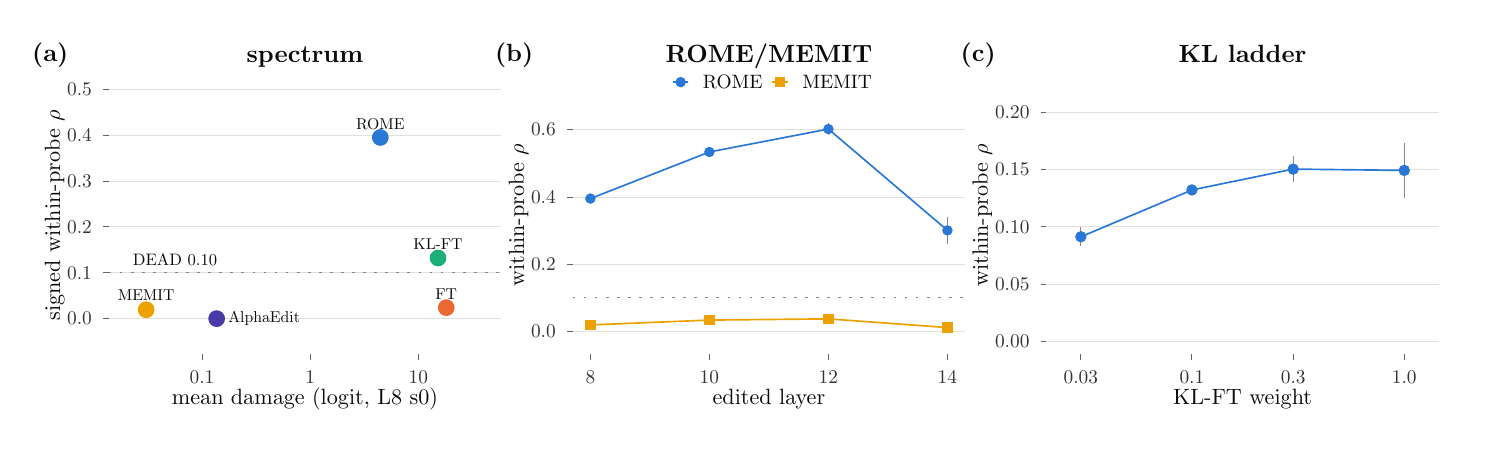
\begin{tikzpicture}[x=1pt,y=1pt]
\definecolor{fillColor}{RGB}{255,255,255}
\path[use as bounding box,fill=fillColor,fill opacity=0.00] (0,0) rectangle (517.45,144.54);
\begin{scope}
\path[clip] (  0.00,  0.00) rectangle (517.45,144.54);
\definecolor{drawColor}{RGB}{255,255,255}
\definecolor{fillColor}{RGB}{255,255,255}

\path[draw=drawColor,line width= 0.6pt,line join=round,line cap=round,fill=fillColor] ( -0.00, -0.00) rectangle (517.45,144.54);
\end{scope}
\begin{scope}
\path[clip] (  5.50,  5.50) rectangle (173.15,139.04);
\definecolor{fillColor}{RGB}{255,255,255}

\path[fill=fillColor] (  5.50,  5.50) rectangle (173.15,139.04);
\end{scope}
\begin{scope}
\path[clip] (173.15,  5.50) rectangle (340.80,139.04);
\definecolor{fillColor}{RGB}{255,255,255}

\path[fill=fillColor] (173.15,  5.50) rectangle (340.80,139.04);
\end{scope}
\begin{scope}
\path[clip] (340.80,  5.50) rectangle (511.95,139.04);
\definecolor{fillColor}{RGB}{255,255,255}

\path[fill=fillColor] (340.80,  5.50) rectangle (511.95,139.04);
\end{scope}
\begin{scope}
\path[clip] ( 29.24, 26.56) rectangle (171.15,126.82);
\definecolor{drawColor}{RGB}{225,224,217}

\path[draw=drawColor,line width= 0.3pt,line join=round] ( 29.24, 39.40) --
	(171.15, 39.40);

\path[draw=drawColor,line width= 0.3pt,line join=round] ( 29.24, 55.98) --
	(171.15, 55.98);

\path[draw=drawColor,line width= 0.3pt,line join=round] ( 29.24, 72.55) --
	(171.15, 72.55);

\path[draw=drawColor,line width= 0.3pt,line join=round] ( 29.24, 89.12) --
	(171.15, 89.12);

\path[draw=drawColor,line width= 0.3pt,line join=round] ( 29.24,105.69) --
	(171.15,105.69);

\path[draw=drawColor,line width= 0.3pt,line join=round] ( 29.24,122.26) --
	(171.15,122.26);
\definecolor{drawColor}{RGB}{137,135,129}

\path[draw=drawColor,line width= 0.3pt,dash pattern=on 1pt off 3pt ,line join=round] ( 29.24, 55.98) -- (171.15, 55.98);
\definecolor{drawColor}{RGB}{11,11,11}

\node[text=drawColor,anchor=base west,inner sep=0pt, outer sep=0pt, scale=  0.60] at ( 38.06, 58.67) {DEAD 0.10};
\definecolor{drawColor}{RGB}{235,104,52}
\definecolor{fillColor}{RGB}{235,104,52}

\path[draw=drawColor,line width= 0.3pt,line join=round,line cap=round,fill=fillColor] (151.26, 43.37) circle (  2.86);
\definecolor{drawColor}{RGB}{27,175,122}
\definecolor{fillColor}{RGB}{27,175,122}

\path[draw=drawColor,line width= 0.3pt,line join=round,line cap=round,fill=fillColor] (148.28, 61.31) circle (  2.86);
\definecolor{drawColor}{RGB}{42,120,214}
\definecolor{fillColor}{RGB}{42,120,214}

\path[draw=drawColor,line width= 0.3pt,line join=round,line cap=round,fill=fillColor] (127.43,104.86) circle (  2.86);
\definecolor{drawColor}{RGB}{237,161,0}
\definecolor{fillColor}{RGB}{237,161,0}

\path[draw=drawColor,line width= 0.3pt,line join=round,line cap=round,fill=fillColor] ( 42.82, 42.62) circle (  2.86);
\definecolor{drawColor}{RGB}{74,58,167}
\definecolor{fillColor}{RGB}{74,58,167}

\path[draw=drawColor,line width= 0.3pt,line join=round,line cap=round,fill=fillColor] ( 68.29, 39.40) circle (  2.86);
\definecolor{drawColor}{RGB}{11,11,11}

\node[text=drawColor,anchor=base,inner sep=0pt, outer sep=0pt, scale=  0.57] at (151.26, 46.33) {FT};

\node[text=drawColor,anchor=base,inner sep=0pt, outer sep=0pt, scale=  0.57] at (148.28, 64.28) {KL-FT};

\node[text=drawColor,anchor=base,inner sep=0pt, outer sep=0pt, scale=  0.57] at (127.43,107.83) {ROME};

\node[text=drawColor,anchor=base,inner sep=0pt, outer sep=0pt, scale=  0.57] at ( 42.82, 45.95) {MEMIT};

\node[text=drawColor,anchor=base west,inner sep=0pt, outer sep=0pt, scale=  0.57] at ( 72.50, 37.92) {AlphaEdit};
\end{scope}
\begin{scope}
\path[clip] (  0.00,  0.00) rectangle (517.45,144.54);
\definecolor{drawColor}{gray}{0.20}

\node[text=drawColor,anchor=base east,inner sep=0pt, outer sep=0pt, scale=  0.70] at ( 23.19, 37.13) {0.0};

\node[text=drawColor,anchor=base east,inner sep=0pt, outer sep=0pt, scale=  0.70] at ( 23.19, 53.70) {0.1};

\node[text=drawColor,anchor=base east,inner sep=0pt, outer sep=0pt, scale=  0.70] at ( 23.19, 70.27) {0.2};

\node[text=drawColor,anchor=base east,inner sep=0pt, outer sep=0pt, scale=  0.70] at ( 23.19, 86.84) {0.3};

\node[text=drawColor,anchor=base east,inner sep=0pt, outer sep=0pt, scale=  0.70] at ( 23.19,103.41) {0.4};

\node[text=drawColor,anchor=base east,inner sep=0pt, outer sep=0pt, scale=  0.70] at ( 23.19,119.98) {0.5};
\end{scope}
\begin{scope}
\path[clip] (  0.00,  0.00) rectangle (517.45,144.54);
\definecolor{drawColor}{gray}{0.40}

\path[draw=drawColor,line width= 0.3pt,line join=round] ( 27.24, 39.40) --
	( 29.24, 39.40);

\path[draw=drawColor,line width= 0.3pt,line join=round] ( 27.24, 55.98) --
	( 29.24, 55.98);

\path[draw=drawColor,line width= 0.3pt,line join=round] ( 27.24, 72.55) --
	( 29.24, 72.55);

\path[draw=drawColor,line width= 0.3pt,line join=round] ( 27.24, 89.12) --
	( 29.24, 89.12);

\path[draw=drawColor,line width= 0.3pt,line join=round] ( 27.24,105.69) --
	( 29.24,105.69);

\path[draw=drawColor,line width= 0.3pt,line join=round] ( 27.24,122.26) --
	( 29.24,122.26);
\end{scope}
\begin{scope}
\path[clip] (  0.00,  0.00) rectangle (517.45,144.54);
\definecolor{drawColor}{gray}{0.40}

\path[draw=drawColor,line width= 0.3pt,line join=round] ( 63.01, 24.56) --
	( 63.01, 26.56);

\path[draw=drawColor,line width= 0.3pt,line join=round] (102.09, 24.56) --
	(102.09, 26.56);

\path[draw=drawColor,line width= 0.3pt,line join=round] (141.17, 24.56) --
	(141.17, 26.56);
\end{scope}
\begin{scope}
\path[clip] (  0.00,  0.00) rectangle (517.45,144.54);
\definecolor{drawColor}{gray}{0.20}

\node[text=drawColor,anchor=base,inner sep=0pt, outer sep=0pt, scale=  0.70] at ( 63.01, 15.96) {0.1};

\node[text=drawColor,anchor=base,inner sep=0pt, outer sep=0pt, scale=  0.70] at (102.09, 15.96) {1};

\node[text=drawColor,anchor=base,inner sep=0pt, outer sep=0pt, scale=  0.70] at (141.17, 15.96) {10};
\end{scope}
\begin{scope}
\path[clip] (  0.00,  0.00) rectangle (517.45,144.54);
\definecolor{drawColor}{RGB}{11,11,11}

\node[text=drawColor,anchor=base,inner sep=0pt, outer sep=0pt, scale=  0.80] at (100.20,  8.23) {mean damage (logit, L8 s0)};
\end{scope}
\begin{scope}
\path[clip] (  0.00,  0.00) rectangle (517.45,144.54);
\definecolor{drawColor}{RGB}{11,11,11}

\node[text=drawColor,rotate= 90.00,anchor=base,inner sep=0pt, outer sep=0pt, scale=  0.80] at ( 11.71, 76.69) {signed within-probe $\rho$};
\end{scope}
\begin{scope}
\path[clip] (  0.00,  0.00) rectangle (517.45,144.54);
\definecolor{drawColor}{RGB}{11,11,11}

\node[text=drawColor,anchor=base,inner sep=0pt, outer sep=0pt, scale=  0.90] at (100.20,131.84) {\bfseries spectrum};
\end{scope}
\begin{scope}
\path[clip] (  0.00,  0.00) rectangle (517.45,144.54);
\definecolor{drawColor}{RGB}{11,11,11}

\node[text=drawColor,anchor=base,inner sep=0pt, outer sep=0pt, scale=  0.90] at (  8.15,132.31) {\bfseries (a)};
\end{scope}
\begin{scope}
\path[clip] (196.89, 26.56) rectangle (338.80,126.82);
\definecolor{drawColor}{RGB}{225,224,217}

\path[draw=drawColor,line width= 0.3pt,line join=round] (196.89, 34.76) --
	(338.80, 34.76);

\path[draw=drawColor,line width= 0.3pt,line join=round] (196.89, 59.07) --
	(338.80, 59.07);

\path[draw=drawColor,line width= 0.3pt,line join=round] (196.89, 83.37) --
	(338.80, 83.37);

\path[draw=drawColor,line width= 0.3pt,line join=round] (196.89,107.68) --
	(338.80,107.68);
\definecolor{drawColor}{RGB}{137,135,129}

\path[draw=drawColor,line width= 0.3pt,dash pattern=on 1pt off 3pt ,line join=round] (196.89, 46.92) -- (338.80, 46.92);

\path[draw=drawColor,line width= 0.4pt,line join=round] (203.34, 84.07) --
	(203.34, 84.07);

\path[draw=drawColor,line width= 0.4pt,line join=round] (203.34, 84.07) --
	(203.34, 81.49);

\path[draw=drawColor,line width= 0.4pt,line join=round] (203.34, 81.49) --
	(203.34, 81.49);

\path[draw=drawColor,line width= 0.4pt,line join=round] (203.34, 37.62) --
	(203.34, 37.62);

\path[draw=drawColor,line width= 0.4pt,line join=round] (203.34, 37.62) --
	(203.34, 36.62);

\path[draw=drawColor,line width= 0.4pt,line join=round] (203.34, 36.62) --
	(203.34, 36.62);

\path[draw=drawColor,line width= 0.4pt,line join=round] (246.34,100.90) --
	(246.34,100.90);

\path[draw=drawColor,line width= 0.4pt,line join=round] (246.34,100.90) --
	(246.34, 98.35);

\path[draw=drawColor,line width= 0.4pt,line join=round] (246.34, 98.35) --
	(246.34, 98.35);

\path[draw=drawColor,line width= 0.4pt,line join=round] (289.35,110.19) --
	(289.35,110.19);

\path[draw=drawColor,line width= 0.4pt,line join=round] (289.35,110.19) --
	(289.35,105.60);

\path[draw=drawColor,line width= 0.4pt,line join=round] (289.35,105.60) --
	(289.35,105.60);

\path[draw=drawColor,line width= 0.4pt,line join=round] (289.35, 40.09) --
	(289.35, 40.09);

\path[draw=drawColor,line width= 0.4pt,line join=round] (289.35, 40.09) --
	(289.35, 38.53);

\path[draw=drawColor,line width= 0.4pt,line join=round] (289.35, 38.53) --
	(289.35, 38.53);

\path[draw=drawColor,line width= 0.4pt,line join=round] (332.35, 76.19) --
	(332.35, 76.19);

\path[draw=drawColor,line width= 0.4pt,line join=round] (332.35, 76.19) --
	(332.35, 66.40);

\path[draw=drawColor,line width= 0.4pt,line join=round] (332.35, 66.40) --
	(332.35, 66.40);
\definecolor{drawColor}{RGB}{42,120,214}

\path[draw=drawColor,line width= 0.6pt,line join=round] (203.34, 82.78) --
	(246.34, 99.62) --
	(289.35,107.90) --
	(332.35, 71.29);
\definecolor{drawColor}{RGB}{237,161,0}

\path[draw=drawColor,line width= 0.6pt,line join=round] (203.34, 37.12) --
	(246.34, 38.88) --
	(289.35, 39.31) --
	(332.35, 36.17);
\definecolor{fillColor}{RGB}{42,120,214}

\path[fill=fillColor] (203.34, 82.78) circle (  1.90);
\definecolor{fillColor}{RGB}{237,161,0}

\path[fill=fillColor] (201.44, 35.22) --
	(205.24, 35.22) --
	(205.24, 39.02) --
	(201.44, 39.02) --
	cycle;
\definecolor{fillColor}{RGB}{42,120,214}

\path[fill=fillColor] (246.34, 99.62) circle (  1.90);
\definecolor{fillColor}{RGB}{237,161,0}

\path[fill=fillColor] (244.45, 36.99) --
	(248.24, 36.99) --
	(248.24, 40.78) --
	(244.45, 40.78) --
	cycle;
\definecolor{fillColor}{RGB}{42,120,214}

\path[fill=fillColor] (289.35,107.90) circle (  1.90);
\definecolor{fillColor}{RGB}{237,161,0}

\path[fill=fillColor] (287.45, 37.41) --
	(291.25, 37.41) --
	(291.25, 41.21) --
	(287.45, 41.21) --
	cycle;
\definecolor{fillColor}{RGB}{42,120,214}

\path[fill=fillColor] (332.35, 71.29) circle (  1.90);
\definecolor{fillColor}{RGB}{237,161,0}

\path[fill=fillColor] (330.45, 34.28) --
	(334.25, 34.28) --
	(334.25, 38.07) --
	(330.45, 38.07) --
	cycle;
\end{scope}
\begin{scope}
\path[clip] (  0.00,  0.00) rectangle (517.45,144.54);
\definecolor{drawColor}{gray}{0.20}

\node[text=drawColor,anchor=base east,inner sep=0pt, outer sep=0pt, scale=  0.70] at (190.84, 32.49) {0.0};

\node[text=drawColor,anchor=base east,inner sep=0pt, outer sep=0pt, scale=  0.70] at (190.84, 56.79) {0.2};

\node[text=drawColor,anchor=base east,inner sep=0pt, outer sep=0pt, scale=  0.70] at (190.84, 81.10) {0.4};

\node[text=drawColor,anchor=base east,inner sep=0pt, outer sep=0pt, scale=  0.70] at (190.84,105.40) {0.6};
\end{scope}
\begin{scope}
\path[clip] (  0.00,  0.00) rectangle (517.45,144.54);
\definecolor{drawColor}{gray}{0.40}

\path[draw=drawColor,line width= 0.3pt,line join=round] (194.89, 34.76) --
	(196.89, 34.76);

\path[draw=drawColor,line width= 0.3pt,line join=round] (194.89, 59.07) --
	(196.89, 59.07);

\path[draw=drawColor,line width= 0.3pt,line join=round] (194.89, 83.37) --
	(196.89, 83.37);

\path[draw=drawColor,line width= 0.3pt,line join=round] (194.89,107.68) --
	(196.89,107.68);
\end{scope}
\begin{scope}
\path[clip] (  0.00,  0.00) rectangle (517.45,144.54);
\definecolor{drawColor}{gray}{0.40}

\path[draw=drawColor,line width= 0.3pt,line join=round] (203.34, 24.56) --
	(203.34, 26.56);

\path[draw=drawColor,line width= 0.3pt,line join=round] (246.34, 24.56) --
	(246.34, 26.56);

\path[draw=drawColor,line width= 0.3pt,line join=round] (289.35, 24.56) --
	(289.35, 26.56);

\path[draw=drawColor,line width= 0.3pt,line join=round] (332.35, 24.56) --
	(332.35, 26.56);
\end{scope}
\begin{scope}
\path[clip] (  0.00,  0.00) rectangle (517.45,144.54);
\definecolor{drawColor}{gray}{0.20}

\node[text=drawColor,anchor=base,inner sep=0pt, outer sep=0pt, scale=  0.70] at (203.34, 15.96) {8};

\node[text=drawColor,anchor=base,inner sep=0pt, outer sep=0pt, scale=  0.70] at (246.34, 15.96) {10};

\node[text=drawColor,anchor=base,inner sep=0pt, outer sep=0pt, scale=  0.70] at (289.35, 15.96) {12};

\node[text=drawColor,anchor=base,inner sep=0pt, outer sep=0pt, scale=  0.70] at (332.35, 15.96) {14};
\end{scope}
\begin{scope}
\path[clip] (  0.00,  0.00) rectangle (517.45,144.54);
\definecolor{drawColor}{RGB}{11,11,11}

\node[text=drawColor,anchor=base,inner sep=0pt, outer sep=0pt, scale=  0.80] at (267.85,  8.23) {edited layer};
\end{scope}
\begin{scope}
\path[clip] (  0.00,  0.00) rectangle (517.45,144.54);
\definecolor{drawColor}{RGB}{11,11,11}

\node[text=drawColor,rotate= 90.00,anchor=base,inner sep=0pt, outer sep=0pt, scale=  0.80] at (179.36, 76.69) {within-probe $\rho$};
\end{scope}
\begin{scope}
\path[clip] (  0.00,  0.00) rectangle (517.45,144.54);
\definecolor{drawColor}{RGB}{42,120,214}

\path[draw=drawColor,line width= 0.6pt,line join=round] (233.16,124.85) -- (238.76,124.85);
\definecolor{fillColor}{RGB}{42,120,214}

\path[fill=fillColor] (235.96,124.85) circle (  1.90);
\end{scope}
\begin{scope}
\path[clip] (  0.00,  0.00) rectangle (517.45,144.54);
\definecolor{drawColor}{RGB}{237,161,0}

\path[draw=drawColor,line width= 0.6pt,line join=round] (269.10,124.85) -- (274.70,124.85);
\definecolor{fillColor}{RGB}{237,161,0}

\path[fill=fillColor] (270.01,122.96) --
	(273.80,122.96) --
	(273.80,126.75) --
	(270.01,126.75) --
	cycle;
\end{scope}
\begin{scope}
\path[clip] (  0.00,  0.00) rectangle (517.45,144.54);
\definecolor{drawColor}{RGB}{11,11,11}

\node[text=drawColor,anchor=base west,inner sep=0pt, outer sep=0pt, scale=  0.70] at (243.96,122.58) {ROME};
\end{scope}
\begin{scope}
\path[clip] (  0.00,  0.00) rectangle (517.45,144.54);
\definecolor{drawColor}{RGB}{11,11,11}

\node[text=drawColor,anchor=base west,inner sep=0pt, outer sep=0pt, scale=  0.70] at (279.90,122.58) {MEMIT};
\end{scope}
\begin{scope}
\path[clip] (  0.00,  0.00) rectangle (517.45,144.54);
\definecolor{drawColor}{RGB}{11,11,11}

\node[text=drawColor,anchor=base,inner sep=0pt, outer sep=0pt, scale=  0.90] at (267.85,131.84) {\bfseries ROME/MEMIT};
\end{scope}
\begin{scope}
\path[clip] (  0.00,  0.00) rectangle (517.45,144.54);
\definecolor{drawColor}{RGB}{11,11,11}

\node[text=drawColor,anchor=base,inner sep=0pt, outer sep=0pt, scale=  0.90] at (175.80,132.31) {\bfseries (b)};
\end{scope}
\begin{scope}
\path[clip] (368.04, 26.56) rectangle (509.95,126.82);
\definecolor{drawColor}{RGB}{225,224,217}

\path[draw=drawColor,line width= 0.3pt,line join=round] (368.04, 31.12) --
	(509.95, 31.12);

\path[draw=drawColor,line width= 0.3pt,line join=round] (368.04, 51.83) --
	(509.95, 51.83);

\path[draw=drawColor,line width= 0.3pt,line join=round] (368.04, 72.55) --
	(509.95, 72.55);

\path[draw=drawColor,line width= 0.3pt,line join=round] (368.04, 93.26) --
	(509.95, 93.26);

\path[draw=drawColor,line width= 0.3pt,line join=round] (368.04,113.98) --
	(509.95,113.98);
\definecolor{drawColor}{RGB}{137,135,129}

\path[draw=drawColor,line width= 0.4pt,line join=round] (380.57, 72.46) --
	(380.57, 72.46);

\path[draw=drawColor,line width= 0.4pt,line join=round] (380.57, 72.46) --
	(380.57, 65.50);

\path[draw=drawColor,line width= 0.4pt,line join=round] (380.57, 65.50) --
	(380.57, 65.50);

\path[draw=drawColor,line width= 0.4pt,line join=round] (420.69, 87.13) --
	(420.69, 87.13);

\path[draw=drawColor,line width= 0.4pt,line join=round] (420.69, 87.13) --
	(420.69, 84.64);

\path[draw=drawColor,line width= 0.4pt,line join=round] (420.69, 84.64) --
	(420.69, 84.64);

\path[draw=drawColor,line width= 0.4pt,line join=round] (457.30, 98.03) --
	(457.30, 98.03);

\path[draw=drawColor,line width= 0.4pt,line join=round] (457.30, 98.03) --
	(457.30, 88.83);

\path[draw=drawColor,line width= 0.4pt,line join=round] (457.30, 88.83) --
	(457.30, 88.83);

\path[draw=drawColor,line width= 0.4pt,line join=round] (497.43,102.79) --
	(497.43,102.79);

\path[draw=drawColor,line width= 0.4pt,line join=round] (497.43,102.79) --
	(497.43, 83.15);

\path[draw=drawColor,line width= 0.4pt,line join=round] (497.43, 83.15) --
	(497.43, 83.15);
\definecolor{drawColor}{RGB}{42,120,214}

\path[draw=drawColor,line width= 0.6pt,line join=round] (380.57, 68.98) --
	(420.69, 85.89) --
	(457.30, 93.43) --
	(497.43, 92.97);
\definecolor{fillColor}{RGB}{42,120,214}

\path[draw=drawColor,line width= 0.3pt,line join=round,line cap=round,fill=fillColor] (380.57, 68.98) circle (  1.90);

\path[draw=drawColor,line width= 0.3pt,line join=round,line cap=round,fill=fillColor] (420.69, 85.89) circle (  1.90);

\path[draw=drawColor,line width= 0.3pt,line join=round,line cap=round,fill=fillColor] (457.30, 93.43) circle (  1.90);

\path[draw=drawColor,line width= 0.3pt,line join=round,line cap=round,fill=fillColor] (497.43, 92.97) circle (  1.90);
\end{scope}
\begin{scope}
\path[clip] (  0.00,  0.00) rectangle (517.45,144.54);
\definecolor{drawColor}{gray}{0.20}

\node[text=drawColor,anchor=base east,inner sep=0pt, outer sep=0pt, scale=  0.70] at (361.99, 28.84) {0.00};

\node[text=drawColor,anchor=base east,inner sep=0pt, outer sep=0pt, scale=  0.70] at (361.99, 49.55) {0.05};

\node[text=drawColor,anchor=base east,inner sep=0pt, outer sep=0pt, scale=  0.70] at (361.99, 70.27) {0.10};

\node[text=drawColor,anchor=base east,inner sep=0pt, outer sep=0pt, scale=  0.70] at (361.99, 90.98) {0.15};

\node[text=drawColor,anchor=base east,inner sep=0pt, outer sep=0pt, scale=  0.70] at (361.99,111.70) {0.20};
\end{scope}
\begin{scope}
\path[clip] (  0.00,  0.00) rectangle (517.45,144.54);
\definecolor{drawColor}{gray}{0.40}

\path[draw=drawColor,line width= 0.3pt,line join=round] (366.04, 31.12) --
	(368.04, 31.12);

\path[draw=drawColor,line width= 0.3pt,line join=round] (366.04, 51.83) --
	(368.04, 51.83);

\path[draw=drawColor,line width= 0.3pt,line join=round] (366.04, 72.55) --
	(368.04, 72.55);

\path[draw=drawColor,line width= 0.3pt,line join=round] (366.04, 93.26) --
	(368.04, 93.26);

\path[draw=drawColor,line width= 0.3pt,line join=round] (366.04,113.98) --
	(368.04,113.98);
\end{scope}
\begin{scope}
\path[clip] (  0.00,  0.00) rectangle (517.45,144.54);
\definecolor{drawColor}{gray}{0.40}

\path[draw=drawColor,line width= 0.3pt,line join=round] (380.57, 24.56) --
	(380.57, 26.56);

\path[draw=drawColor,line width= 0.3pt,line join=round] (420.69, 24.56) --
	(420.69, 26.56);

\path[draw=drawColor,line width= 0.3pt,line join=round] (457.30, 24.56) --
	(457.30, 26.56);

\path[draw=drawColor,line width= 0.3pt,line join=round] (497.43, 24.56) --
	(497.43, 26.56);
\end{scope}
\begin{scope}
\path[clip] (  0.00,  0.00) rectangle (517.45,144.54);
\definecolor{drawColor}{gray}{0.20}

\node[text=drawColor,anchor=base,inner sep=0pt, outer sep=0pt, scale=  0.70] at (380.57, 15.96) {0.03};

\node[text=drawColor,anchor=base,inner sep=0pt, outer sep=0pt, scale=  0.70] at (420.69, 15.96) {0.1};

\node[text=drawColor,anchor=base,inner sep=0pt, outer sep=0pt, scale=  0.70] at (457.30, 15.96) {0.3};

\node[text=drawColor,anchor=base,inner sep=0pt, outer sep=0pt, scale=  0.70] at (497.43, 15.96) {1.0};
\end{scope}
\begin{scope}
\path[clip] (  0.00,  0.00) rectangle (517.45,144.54);
\definecolor{drawColor}{RGB}{11,11,11}

\node[text=drawColor,anchor=base,inner sep=0pt, outer sep=0pt, scale=  0.80] at (439.00,  8.23) {KL-FT weight};
\end{scope}
\begin{scope}
\path[clip] (  0.00,  0.00) rectangle (517.45,144.54);
\definecolor{drawColor}{RGB}{11,11,11}

\node[text=drawColor,rotate= 90.00,anchor=base,inner sep=0pt, outer sep=0pt, scale=  0.80] at (347.01, 76.69) {within-probe $\rho$};
\end{scope}
\begin{scope}
\path[clip] (  0.00,  0.00) rectangle (517.45,144.54);
\definecolor{drawColor}{RGB}{11,11,11}

\node[text=drawColor,anchor=base,inner sep=0pt, outer sep=0pt, scale=  0.90] at (439.00,131.84) {\bfseries KL ladder};
\end{scope}
\begin{scope}
\path[clip] (  0.00,  0.00) rectangle (517.45,144.54);
\definecolor{drawColor}{RGB}{11,11,11}

\node[text=drawColor,anchor=base,inner sep=0pt, outer sep=0pt, scale=  0.90] at (343.48,132.31) {\bfseries (c)};
\end{scope}
\end{tikzpicture}
